\section{Experiments for Proposal 1}\label{section:experiment_part_1}

In this section we present the results of experiments we conducted in order to empirically ascertain the difference in performance of several multi-label ranking methods, applied to social tag prediction, as detailed in Chapter \ref{chap:proposal}.

\subsection{TF-IDF weighted Bag-of-words Features, Binary Relevance + Linear SVM Classifier}

In this experiment, we apply the commonly-used \textit{Binary Relevance}\footnote{As previously noted, this method is also called \textit{One-vs-Rest} because one classifier is trained for each separate category, or label.} meta-estimator \citep{tsoumakas_katakis_2007} using a linear SVM classifier as underlying model.

This is a commonly-used technique for social tag prediction, as seen in \cite{chen_etal_2008, goh_etal_2008,illig_etal_2011,tao_yao_2016} among others.

\subsubsection{Results on Dataset 1}

\begin{figure}[H]
    \centering
    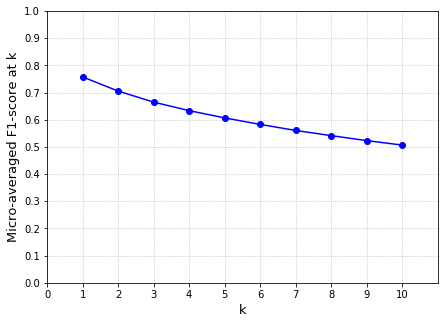
\includegraphics[width=7cm]{chapters/05_experiments/images/svm-tf-idf-delicious-20-frac.png}
    \caption{Results of applying Binary Relevance + Linear SVM with TF-IDF features on the Delicious t-140 Dataset (validation set scores shown)}
    \label{fig:ovr_svm_movielens}
\end{figure}

\subsubsection{Results on Dataset 2}

\begin{figure}[H]
    \centering
    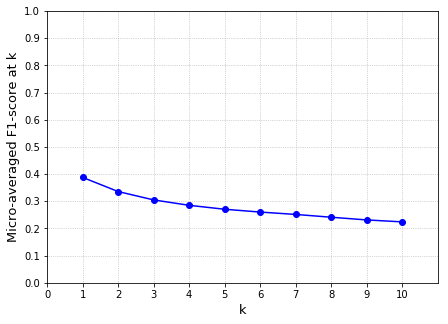
\includegraphics[width=7cm]{chapters/05_experiments/images/svm-tf-idf-movielens.png}
    \caption{Results of applying Binary Relevance + Linear SVM with TF-IDF features on the Movielens Dataset (validation set scores shown)}
    \label{fig:ovr_svm_movielens}
\end{figure}

\subsubsection{Discussion}

\begin{figure}[H]
    \centering
    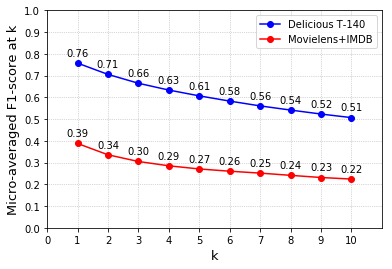
\includegraphics[width=7cm]{chapters/05_experiments/images/proposal-1-compared-ovr-svm-bow.png}
    \caption{Binary Relevance, Linear SVM with TF-IDF features: Compared results (validation set scores)}
    \label{fig:compared_ovr_svm}
\end{figure}

As expected, the results in Dataset 1 were far better than those for Dataset 2, due to the differences in the tag distribution for both datasets.

It is interesting to note that the decrease in scores for Dataset 1 is somewhat more pronounced than in Dataset 2.

\subsection{TF-IDF weighted Bag-of-words Features, k-Nearest Neighbours Classifier}

The $k$-Nearest Neighbors is a very popular machine learning method that can be used both for classification and for regression. It consists in simply calculating the distances (assuming an $n$-dimensional representations) to every other instance, at \textit{inference time}\footnote{Methods such as $k$-NN are called \textit{lazy} methods because they need no training, as they defer all processing until actual inference is made.}. Then, each neighbor up to $k$ is treated as a source of information to help predict the class for the query instance. 

With respect to tag prediction, multiple (\cite{martinez_etal_2009,chidlovskii_2012,zhang_etal_2015,charte_etal_2015}\footnote{\cite{charte_etal_2015} have applied an approach very similar to ours, namely using multi-label $k$-NN to classify text into multiple tags, using TF-IDF representation. } to cite but a few) authors have applied some form of neighbor-based classifier to predicting tags for a query resource. 

In general, they proceed by finding nearest neighbors based on the resource's vector representation, as per the usual algorithm. Then, each neighbor's binary tag vector is added up and tags which are more commonly seen in the query instance's neighborhood are suggested.

Since we only want to use this method as a baseline, we implemented the most basic version thereof, namely simple, unweighted $k$-NN. Furthermore, we ran grid search over the method's hyperparameters, namely $k$, the number of neighbors to consider and also over the distance metric to use (cosine, euclidean, manhattan, etc).

\subsubsection{Results on dataset 1}

\begin{figure}[H]
    \centering
    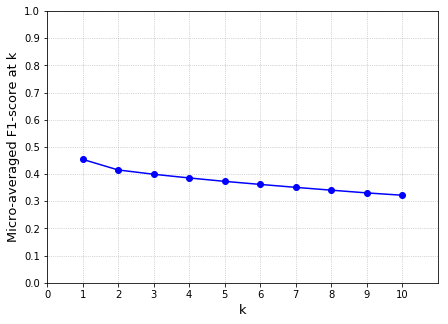
\includegraphics[width=7cm]{chapters/05_experiments/images/knn-tfidf-delicious.png}
    \caption{Applying $k$-NN on the Delicious Dataset, using TF-IDF weighted bag-of-words representation (validation set scores shown)}
    \label{fig:knn__movielens}
\end{figure}

\subsubsection{Results on Dataset 2}

\begin{figure}[H]
    \centering
    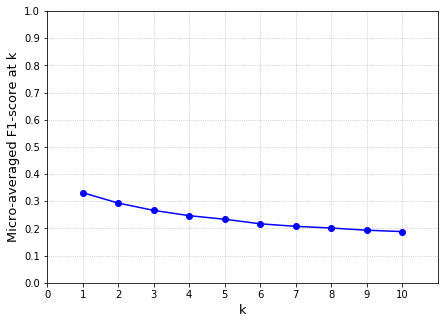
\includegraphics[width=7cm]{chapters/05_experiments/images/knn-tfidf-movielens.png}
    \caption{Applying $k$-NN on the Movielens Dataset, using TF-IDF weighted bag-of-words representation (validation set scores shown)}
    \label{fig:knn__movielens}
\end{figure}

\subsubsection{Discussion}

\begin{figure}[H]
    \centering
    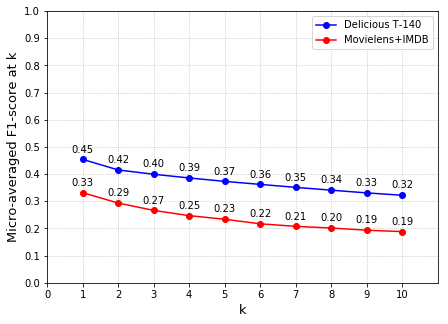
\includegraphics[width=7cm]{chapters/05_experiments/images/proposal-1-compared-knn-tfidf.png}
    \caption{$k$-NN with TF-IDF features: Compared results (validation set scores)}
    \label{fig:compared_ovr_svm}
\end{figure}

Although the results were satisfactory, one can see that the difference in performance on both datasets is not as large as in the previous example. One reason for that may be that the large number of neighbours (found by model selection via grid search) may act as a regularizer, decreasing the variance on out-of-sample examples but at the cost of a higher bias.

 We would like to note that, surprisingly, using a \textit{weighted} variant did not increase performance on this task. In other words, weighing the contribution by the inverse of the distance to each neighbor did not increase the accuracy of the model.

\subsection{TF-IDF weighted Bag-of-words Features, Topic Distances}

In this approach, which has been suggested by \cite{choubey_2011},we first train a topic model on train set documents using Latent Dirichlet Allocation (LDA) (\cite{blei_etal_2003}). Then, at query time, we calculate the topic distribution for the query document and also the single most similar train set document, as measured by the Kullback-Leibler Divergence (KL-Divergence, \cite{kullback_leibler_1951}) between the topic distributions of the documents. Finally, the tags used in the found document are used as suggestions for the unlabelled query document.

\subsubsection{Results on dataset 1}

\begin{figure}[H]
    \centering
    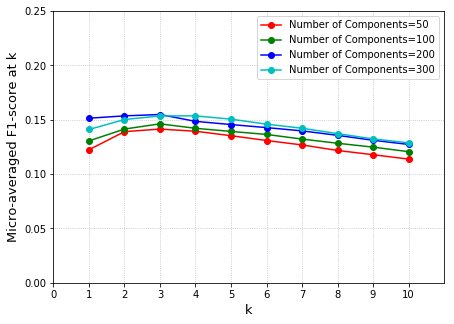
\includegraphics[width=7cm]{chapters/05_experiments/images/delicious-topic-distances.png}
    \caption{Applying Topic Distances on the Delicious Dataset, with varying values for the choice of LDA components}
    \label{fig:topic_distances_delicious}
\end{figure}

\begin{figure}[H]
    \centering
    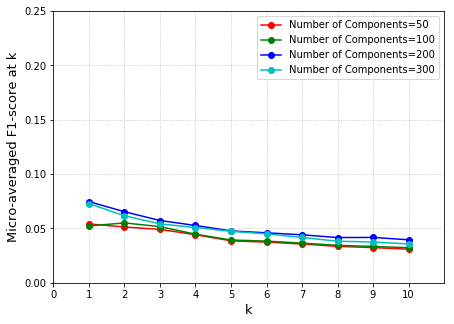
\includegraphics[width=7cm]{chapters/05_experiments/images/movielens-topic-distances.png}
    \caption{Applying Topic Distances on the Movielens Dataset, with varying values for the choice of LDA components}
    \label{fig:topic_distances_movielens}
\end{figure}

\subsubsection{Discussion}

\begin{figure}[H]
    \centering
    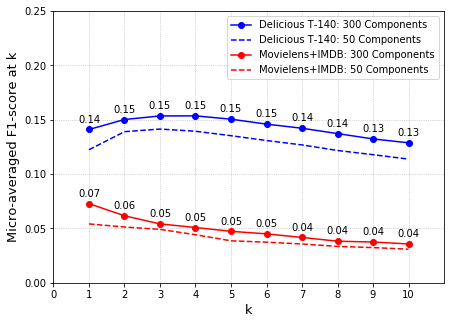
\includegraphics[width=7cm]{chapters/05_experiments/images/proposal-1-compared-topic-distances.png}
    \caption{Topic Distances: Compared results (validation set scores). Best and worst results for each Dataset shown for comparison.}
    \label{fig:compared_topic_distances}
\end{figure}

While the results were overall worse than previous classifiers, the overall pattern of dataset 1 (Delicious) performing better than dataset 2 was maintained. Notably, however, the difference is now much more pronounced (in relative terms), standing at up to 300\%.

It is worth mentioning that the results achieved are close to what the original authors', lending credibility to the fact that this method performs very poorly overall, not just on specific datasets and/or specific conditions.

\subsection{TF-IDF weighted Bag-of-words Features, Topic Words}

In this approach, also suggested by \cite{choubey_2011}, one trains an LDA topic model on documents in the train set. At test time, the topic distribution for each query document is calculated with the trained model. Then, the most representative words\footnote{Only words that are in the actual tag vocabulary are used.} for the most representative topic are suggested as tags for the query document.

\subsubsection{Results on dataset 1}

\begin{figure}[H]
    \centering
    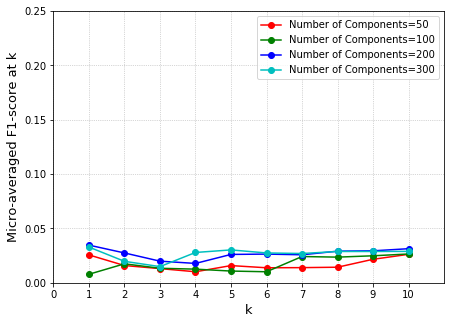
\includegraphics[width=7cm]{chapters/05_experiments/images/delicious-topic-words.png}
    \caption{Applying Topic Words on the Delicious Dataset, with varying values for the choice of LDA components (validation set scores shown)}
    \label{fig:topic_words_delicious}
\end{figure}

\subsubsection{Results on Dataset 2}

\begin{figure}[H]
    \centering
    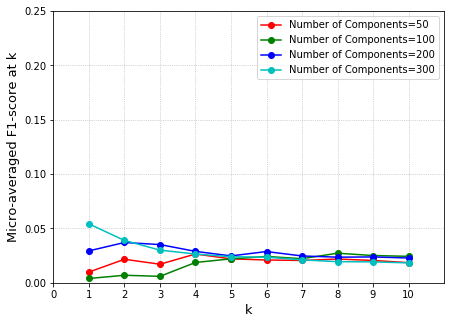
\includegraphics[width=7cm]{chapters/05_experiments/images/movielens-topic-words.png}
    \caption{Applying Topic Words on the Movielens Dataset, with varying values for the choice of LDA components (validation set scores shown)}
    \label{fig:topic_words_movielens}
\end{figure}

\subsubsection{Discussion}

\begin{figure}[H]
    \centering
    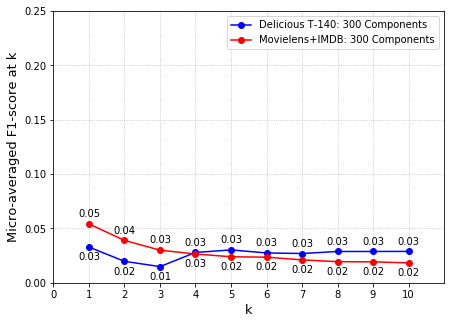
\includegraphics[width=7cm]{chapters/05_experiments/images/proposal-1-compared-topic-words.png}
    \caption{Topic Words: Compared results (validation set scores) using the best choice for the number of components.}
    \label{fig:compared_topic_words}
\end{figure}

Once again, the results are not very good (in comparison to classifiers such as SVM, used previously). These, however, resemble results in the original source \citep{choubey_2011}. Notably, there doesn't seem to be any consistent difference when one dataset is compared to another, or as $k$ grows. This may indicate that this method is not effectively learning much.

\subsection{LDA Topic Probabilities, k-nearest Neighbours Classifier}\label{sub:lda_topics}

Although Latent Dirichlet Allocation (LDA) \citep{blei_etal_2003} was originally created as a means to infer representative words for topics in corpora, it can be (and frequently is) used to extract features for documents. In fact, this approach was used and suggested in the original paper itself.

In other words, LDA can be used as a form of dimensionality reduction to reduce the size of feature vectors\footnote{Assuming an original bag-of-words representation without trimming the number of words used.} from $V$ to $k$, respectively the vocabulary size and the number of components in the LDA model.

Using these topic probabilities as features, we can then proceed onto classifying the documents using any classifier we wish. We have chose to use two classifier for this task: \textbf{a)} a simple $k$-nearest Neighbours Classifier so as to enable comparison between using LDA features and using bag-of-words features and \textbf{b)} (in the next subsection) an SVM classifier, as suggested in the original LDA article.

\subsubsection{Results on dataset 1}

\begin{figure}[H]
    \centering
    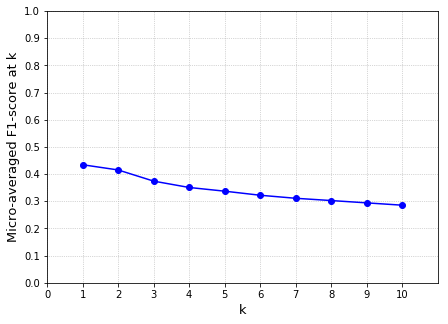
\includegraphics[width=7cm]{chapters/05_experiments/images/knn-lda-delicious.png}
    \caption{k-Nearest Neighbor classifier on the Delicious dataset, using LDA topic probabilities as features (validation set scores shown).}
    \label{fig:knn_lda_delicious}
\end{figure}

\subsubsection{Results on Dataset 2}

\begin{figure}[H]
    \centering
    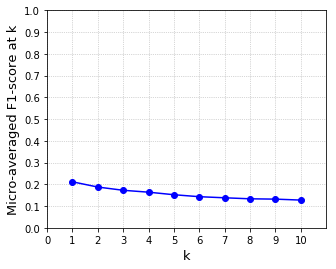
\includegraphics[width=7cm]{chapters/05_experiments/images/knn-lda-movielens.png}
    \caption{k-Nearest Neighbor classifier on the Movielens dataset, using LDA topic probabilities as features (validation set scores shown).}
    \label{fig:knn_lda_movielens}
\end{figure}

\subsubsection{Discussion}

\begin{figure}[H]
    \centering
    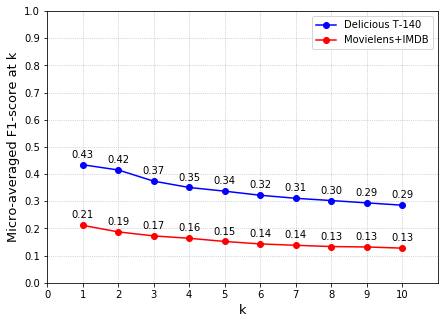
\includegraphics[width=7cm]{chapters/05_experiments/images/proposal-1-compared-knn-lda.png}
    \caption{$k$-NN using LDA features: Compared results (validation set scores).}
    \label{fig:compared_knn_lda}
\end{figure}

It is interesting to note that, although only 50 components are used in this setup, we get 0.43 as F-1 score, compared with 0.45 when using $k$-NN with 500-dimensional bag-of-words features. In other words, we were able to reduce the dimensionality\footnote{Therefore also reducing the training and testing time, processing power needed, not to mention better generalization due to using a less complex model.} of the problem while losing just a bit of performance.  

Interestingly, however, the compared results for the second dataset, namely, Movielens+IMDB, was markedly worse; 0.21 using LDA features vs 0.33 using bag-of-words features.

\subsection{LDA Topic Probabilities, SVM classifier}

As mentioned on the previous subsection, we will compare results between both datasets using LDA as a simple dimensionality reduction step on top of TF-IDF weighted bag-of-words features. We will use an SVM classifier, as suggested in the original LDA paper by \cite{blei_etal_2003}.

However, since the features are now of a \textit{denser} nature, we will add other types of kernels to the hyperparameter search space, namely Radial Basis Function (RBF) and a also a polynomial kernel, in addition to the default linear kernel.

\subsubsection{Results on dataset 1}

\begin{figure}[H]
    \centering
    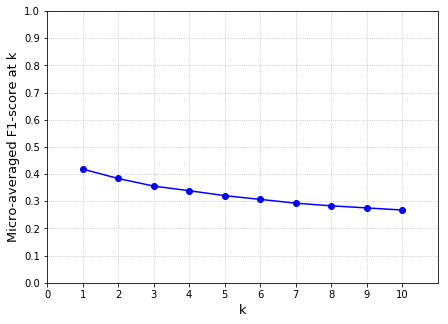
\includegraphics[width=7cm]{chapters/05_experiments/images/svm-lda-delicious.png}
    \caption{SVM classifier on the Delicious dataset, using LDA topic probabilities as features (validation set scores shown).}
    \label{fig:svm_lda_delicious}
\end{figure}

\subsubsection{Results on Dataset 2}

\begin{figure}[H]
    \centering
    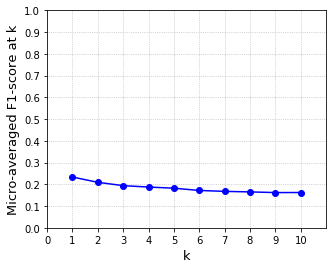
\includegraphics[width=7cm]{chapters/05_experiments/images/svm-lda-tf-idf-movielens.png}
    \caption{SVM classifier on the Movielens dataset, using LDA topic probabilities as features (validation set scores shown).}
    \label{fig:svm_lda_movielens}
\end{figure}

\subsubsection{Discussion}

\begin{figure}[H]
    \centering
    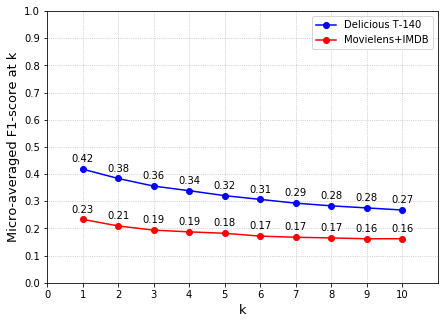
\includegraphics[width=7cm]{chapters/05_experiments/images/proposal-1-compared-svm-lda.png}
    \caption{SVM using LDA features: Compared results (validation set scores).}
    \label{fig:compared_svm_lda}
\end{figure}

Once again, we see that the difference in outcomes is large, of up to 80\%. This is surprising in light of the fact that the best results for each dataset (as obtained via grid search) used just 5 LDA components.

In other words, we were able to provide good performance for this experiment setup using a mere 5 dimensional in place of the original 500 dimensions of the bag-of-words vectors. Note that an RBF kernel was used in this section.

\subsection{Final Results and discussion}

\begin{figure}[H]
    \begin{subfigure}{0.5\textwidth}
        \centering
    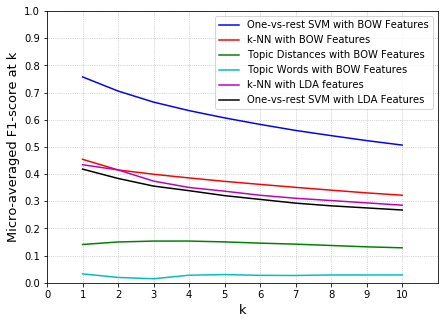
\includegraphics[width=0.8\textwidth]{chapters/05_experiments/images/full-comparison-dataset-1.png}
    \caption{Full comparison of all techniques used on dataset 1: Delicious T-140.}
    \label{fig:full_comparison_dataset_1}
    \end{subfigure}
    \begin{subfigure}{0.5\textwidth}
        \centering
    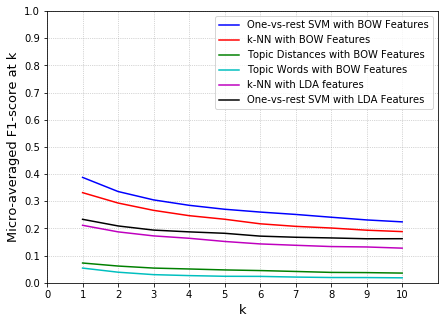
\includegraphics[width=0.8\textwidth]{chapters/05_experiments/images/full-comparison-dataset-2.png}
    \caption{Full comparison of all techniques used on dataset 2: Movielens+IMDB.}
    \label{fig:full_comparison_dataset_2}
    \end{subfigure}
    \caption{Full comparison of all techniques used (validation set scores).}
\end{figure}

As we had initially expected, results in dataset 1 far outperform those in dataset 2, Delicious T-140 and Movielens+IMDB respectively.

\begin{table}[H]
\centering
\caption{Compared dataset statistics}
\begin{tabular}{|c|c|c|}
\hline
\specialcell{} & \textbf{Delicious T-140} & \textbf{Movielens+IMDB} \\
\hline
\specialcell{Total number of Resources} & 147,716 & 6,710 \\
\hline
% \specialcell{Total number of unique tags} & \,\,\, 2,138 \\
% \hline
% \specialcell{Average number of tags per resource} & \,\,\, 12.21 \\
% \hline
% \specialcell{Minimum number of tags per resource} & \,\,\, 1 \\
% \hline
% \specialcell{Maximum number of tags per resource} & \,\,\, 189 \\
% \hline
% \specialcell{Average number of resources per tag} & \,\,\, 38.33 \\
% \hline
% \specialcell{Minimum number of resources per tag} & \,\,\, 10 \\
% \hline
% \specialcell{Maximum number of resources per tag} & \,\,\, 854\\
% \hline
\end{tabular}
\label{tab:dataset_statistics_delicious}
\end{table}

{\color{red} TODO: finish table}

The experiments seem to confirm the intuitive explanation that dataset characteristics do indeed affect the performance of classifiers, at least when measured with our metric of choice (micro-F1 @k).

Intuitively, we could claim that the results were better in dataset 1 because number of resources is much larger (there are many more examples to learn from), the tag vocabulary is smaller (there are less tags to choose from at each prediction) and the number of tags assigned to each resource is capped at 25.

Another possible explanation is that documents in dataset 1 represent the resource itself (a webpage) while in dataset 2 the documents are but a \textit{description} of the resource, not the resource itself (resources are movies). In a way, dataset 2 contains \textit{secondhand information} about the resource.

In addition to the above, dataset 2 is a mixture of two different sources\footnote{See subsection \ref{subsec:dataset_2} for a detailed explanation.}, namely Movielens for the tags and IMDB for the movie plot summary. This may have had an additional effect on lowering the performance of the classifiers since there is a potential mismatch between the two sources.
